% XGBoost Category-Level Feature Ablation
% Replaces: tab:xgboost-category-ablation in appendix_c
% Horizontal bar chart showing MAE degradation when each category is removed

\begin{figure}[htbp]
\centering
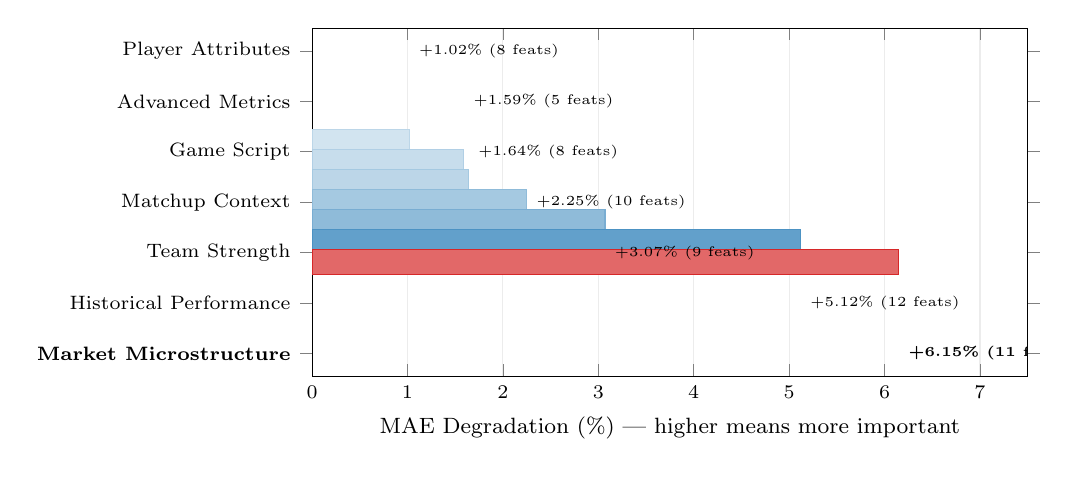
\begin{tikzpicture}
\definecolor{accent}{RGB}{31,119,180}
\definecolor{accentRed}{RGB}{214,39,40}

\begin{axis}[
  width=0.88\textwidth,
  height=6cm,
  xbar,
  bar width=9pt,
  xmin=0, xmax=7.5,
  xlabel={MAE Degradation (\%) --- higher means more important},
  xlabel style={font=\footnotesize},
  ytick={1,2,3,4,5,6,7},
  yticklabels={
    Player Attributes,
    Advanced Metrics,
    Game Script,
    Matchup Context,
    Team Strength,
    Historical Performance,
    {\textbf{Market Microstructure}}
  },
  yticklabel style={font=\scriptsize},
  y dir=reverse,
  xticklabel style={font=\scriptsize},
  grid=major,
  grid style={gray!15},
  xmajorgrids=true,
  ymajorgrids=false,
  enlarge y limits={abs=0.45},
]

% Bars with gradient intensity by importance
\addplot[fill=accent!20, draw=accent!30] coordinates {(1.02, 1)};
\addplot[fill=accent!25, draw=accent!35] coordinates {(1.59, 2)};
\addplot[fill=accent!30, draw=accent!40] coordinates {(1.64, 3)};
\addplot[fill=accent!40, draw=accent!50] coordinates {(2.25, 4)};
\addplot[fill=accent!50, draw=accent!60] coordinates {(3.07, 5)};
\addplot[fill=accent!70, draw=accent!80] coordinates {(5.12, 6)};
\addplot[fill=accentRed!70, draw=accentRed] coordinates {(6.15, 7)};

% Value labels
\node[font=\tiny, anchor=west] at (axis cs:1.02,1) {+1.02\% (8 feats)};
\node[font=\tiny, anchor=west] at (axis cs:1.59,2) {+1.59\% (5 feats)};
\node[font=\tiny, anchor=west] at (axis cs:1.64,3) {+1.64\% (8 feats)};
\node[font=\tiny, anchor=west] at (axis cs:2.25,4) {+2.25\% (10 feats)};
\node[font=\tiny, anchor=west] at (axis cs:3.07,5) {+3.07\% (9 feats)};
\node[font=\tiny, anchor=west] at (axis cs:5.12,6) {+5.12\% (12 feats)};
\node[font=\tiny\bfseries, anchor=west] at (axis cs:6.15,7) {+6.15\% (11 feats)};

\end{axis}
\end{tikzpicture}
\caption[Feature category ablation]{XGBoost feature category ablation (2023--2024, $n=1{,}124$ QB-games). Market microstructure features are most important (+6.15\% MAE degradation when removed), followed by historical performance (+5.12\%). Player attributes are least informative (+1.02\%), suggesting position and experience add minimal signal conditional on performance metrics.}
\label{fig:category-ablation-chart}
\end{figure}
